\section{Implementation}

\begin{frame}
	\frametitle{The Barnes-Hut Approximation}
	\begin{enumerate}
		\item Place all the particles in a tree.
		\item For each tree node, compute the center of mass.
		\item For each particle, compute a force. Start interacting with the root level, request deeper levels if
		$$\theta<\frac{s}{d}.$$
		\item Perform a time step.
		\item \emph{Update} the tree structure.
		\item Save results if needed, go to 2 or exit.
	\end{enumerate}
\end{frame}

\begin{frame}
	\frametitle{The Barnes-Hut Approximation: Tree Construction}
	\begin{figure}
		\centering
		\begin{tikzpicture}[scale=0.05,%
		every circle node/.style = {width=3,fill=black}]
		\input{incl/bh-grid-build.tex}
		\end{tikzpicture}
		\caption{Sample 4-level Barnes-Hut grid with 10 particles.}
		\label{fig:bh-grid}
	\end{figure}
\end{frame}

\begin{frame}
	\frametitle{The Barnes-Hut Approximation: Tree Construction (Cont.)}
	\begin{figure}
		\centering
		\newlength{\lvld}
		\setlength{\lvld}{7em}
		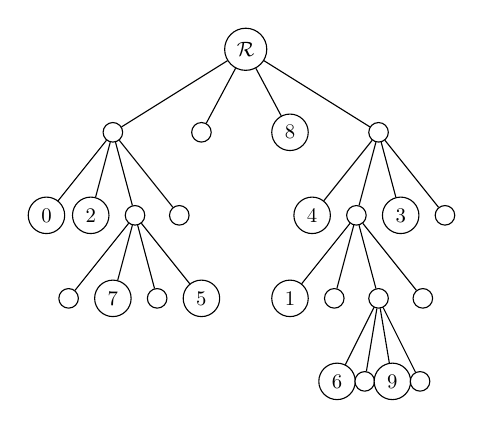
\begin{tikzpicture}[level distance=3em,
		sibling distance=3em,
		level 1/.style={sibling distance=0.80\lvld},
		level 2/.style={sibling distance=0.40\lvld},
		level 3/.style={sibling distance=0.4\lvld},
		level 4/.style={sibling distance=0.25\lvld},
		every node/.style = {shape=circle, draw, align=center, color=black,
			fill=white, scale=0.75}]
		\node {$\mathcal{R}$} %Root
child { node {} %1SW
	child { node{0} } %2SW
	child { node{2} } %2NW
	child { node{} %2SE
		child { node{} } %3SW
		child { node{7} } %3NW
		child { node{} } %3SE
		child { node{5} } } %3NE
	child { node{} } } %2NE
child { node{} }%1NW
child { node{8} }%1SE
child { node{} %1NE
	child { node{4} } %2SW
	child { node{} %2NW
		child { node {1} } %3SW
		child { node {} } %3NW
		child { node {} %3SE
			child { node{6} } %4SW
			child { node{} } %4NW
			child { node{9} } %4SE
			child { node{} } %4SW
		}
		child { node {} } }%3NE
	child { node{3} } %2SE
	child{ node{} } }; %2NE
		\end{tikzpicture}
		\caption{Tree structure associated to the configuration depicted in \cref{fig:bh-grid}.}
		\label{fig:bh-tree}
	\end{figure}
\end{frame}

\begin{frame}
	\frametitle{The Barnes-Hut Approximation: Force Computation}
	\begin{figure}
		\centering
		\begin{tikzpicture}[scale=0.035,%
		every circle node/.style = {width=3,fill=black}]
			% Simulation domain
\only<1,3->{\draw[thick] (0,0) rectangle (100,100);}
\only<2>{\draw[thick,fill=red!20!white] (0,0) rectangle (100,100);}
% Level 1
\draw[thick] (50,0) -- (50,100);
\draw[thick] (0,50) -- (100,50);
\only<3>{\draw[thick,fill=red!20!white] (0,0) rectangle (50,50);}
\only<12>{\draw[thick,fill=red!20!white] (0,50) rectangle (50,100);}
\only<13>{\draw[thick,fill=green!20!white] (50,0) rectangle (100,50);}
\only<14>{\draw[thick,fill=green!20!white] (50,50) rectangle (100,100);}
% Level 2
\draw (0,25) -- (100,25);
\draw (75,0) -- (75,100);
\draw (25,0) -- (25,50);
\draw (50,75)-- (100,75);
\only<4>{\draw[fill=red!20!white] (0,0) rectangle (25,25);}
\only<5>{\draw[fill=green!20!white] (0,25) rectangle (25,50);}
\only<6>{\draw[fill=red!20!white] (25,0) rectangle (50,25);}
\only<11>{\draw[fill=red!20!white] (25,25) rectangle (50,50);}
% Level 3
\draw (25,12.5) -- (50,12.5);
\draw (37.5,0)  -- (37.5,25);
\draw (62.5,75) -- (62.5,100);
\draw (50,87.5) -- (75,87.5);
\only<7>{\draw[fill=red!20!white] (25,0) rectangle (37.5,12.5);}
\only<8>{\draw[fill=green!20!white] (25,12.5) rectangle (37.5,25);}
\only<9>{\draw[fill=green!20!white] (37.5,0) rectangle (50,12.5);}
\only<10>{\draw[fill=red!20!white] (37.5,12.5) rectangle (50,25);}
% Level 4
\draw[thin] (68.625,75) -- (68.625,87.5);
\draw[thin] (62.5,81.125) -- (75,81.125);
% Particles (by increasing id)
\draw[fill=red] (16.9664,19.6802) circle (1); %0
\draw[fill] (54.4110,82.9573) circle (1); %1
\draw[fill] (03.4614,30.2489) circle (1); %2
\draw[fill] (81.4564,52.3018) circle (1); %3
\draw[fill](59.5102,62.4865) circle (1);  %4
\draw[fill] (40.5800,00.4751) circle (1); %5
\draw[fill] (64.4035,77.5371) circle (1); %6
\draw[fill] (36.6343,21.2396) circle (1); %7
\draw[fill] (99.9970,20.3979) circle (1); %8
\draw[fill] (70.6045,79.4802) circle (1); %9
		\end{tikzpicture}
		\hspace*{5pt}
		\setlength{\lvld}{4em}
		\begin{tikzpicture}[scale=0.7,
		level distance=3em,
		sibling distance=3em,
		level 1/.style={sibling distance=0.90\lvld},
		level 2/.style={sibling distance=0.50\lvld},
		level 3/.style={sibling distance=0.5\lvld},
		level 4/.style={sibling distance=0.4\lvld},
		every node/.style = {shape=circle, draw, align=center, color=black,
			fill=white, scale=0.75}]
		\node[onslide=<2>{coarse}]{$\mathcal{R}$}%Root
child { node[onslide=<3>{coarse}]{} %1SW
	child { node[onslide=<4>{coarse}]{0} } %2SW
	child { node[onslide=<5>{detail}]{2} } %2NW
	child { node[onslide=<6>{coarse}]{} %2SE
		child { node[onslide=<7>{coarse}]{} } %3SW
		child { node[onslide=<8>{detail}]{7} } %3NW
		child { node[onslide=<9>{detail}]{5} } %3SE
		child { node[onslide=<10>{coarse}]{} } } %3NE
	child { node[onslide=<11>{coarse}]{} } } %2NE
child { node[onslide=<12>{coarse}]{} }%1NW
child { node[onslide=<13>{detail}]{8} }%1SE
child { node[onslide=<14>{detail}]{} %1NE
	child { node{4} } %2SW
	child { node{} %2NW
		child { node {1} } %3SW
		child { node {} } %3NW
		child { node {} %3SE
			child { node{6} } %4SW
			child { node{} } %4NW
			child { node{9} } %4SE
			child { node{} } %4SW
		}
		child { node {} } }%3NE
	child { node{3} } %2SE
	child{ node{} } }; %2NE
		\end{tikzpicture}
		\caption{Hypothetical force computation for one particle of the system, \cref{fig:bh-grid,fig:bh-tree}.}
		\label{fig:bh-grid-forces}
	\end{figure}
\end{frame}

\begin{frame}
\frametitle{The Barnes-Hut Approximation: Tree Update}
\begin{figure}
	\centering
	\begin{tikzpicture}[scale=0.035,%
	every circle node/.style = {width=3,fill=black}]
	\input{incl/bh-grid-update.tex}
	\end{tikzpicture}
	\hspace*{5pt}
	\setlength{\lvld}{4em}
	\begin{tikzpicture}[scale=0.7,
	level distance=3em,
	sibling distance=3em,
	level 1/.style={sibling distance=0.90\lvld},
	level 2/.style={sibling distance=0.50\lvld},
	level 3/.style={sibling distance=0.5\lvld},
	level 4/.style={sibling distance=0.4\lvld},
	every node/.style = {shape=circle, draw, align=center, color=black,
		fill=white, scale=0.75}]
	\only<1-5>{%
\node {$\mathcal{R}$} %Root
child { node[onslide=<3>{detail}]{} %1SW
	child { node{0} } %2SW
	child { node[onslide=<2>{coarse}]{\only<1-5>{2}} } %2NW
	child { node[onslide=<4>{detail}]{} %2SE
		child { node{} } %3SW
		child { node[onslide=<5-6>{detail}]{7} } %3NW
		child { node{5} } %3SE
		child { node{} } } %3NE
	child { node{} } } %2NE
child { node{} }%1NW
child { node{8} }%1SE
child { node{} %1NE
	child { node{4} } %2SW
	child { node{} %2NW
		child { node {1} } %3SW
		child { node {} } %3NW
		child { node {} %3SE
			child { node{6} } %4SW
			child { node{} } %4NW
			child { node{9} } %4SE
			child { node{} } %4SW
		}
		child { node {} } }%3NE
	child { node{3} } %2SE
	child{ node{} } }; %2NE
}

\only<6->{%
\node {$\mathcal{R}$} %Root
child { node[onslide=<3>{detail}]{} %1SW
	child { node{0} } %2SW
	child { node[onslide=<2>{coarse}]{\only<1-6>{2}} } %2NW
	child { node[onslide=<4>{detail}]{} %2SE
		child { node{} } %3SW
		child { node[onslide=<5-6>{detail}]{}
			child { node{} } %4SW
			child { node[onslide=<7>{detail}]{\only<7>{2}} } %4NW
			child { node{} } %4SE
			child { node{7} } %4NE
		} %3NW
		child { node{5} } %3SE
		child { node{} } } %3NE
	child { node{} } } %2NE
child { node{} }%1NW
child { node{8} }%1SE
child { node{} %1NE
	child { node{4} } %2SW
	child { node{} %2NW
		child { node {1} } %3SW
		child { node {} } %3NW
		child { node {} %3SE
			child { node{6} } %4SW
			child { node{} } %4NW
			child { node{9} } %4SE
			child { node{} } %4SW
		}
		child { node {} } }%3NE
	child { node{3} } %2SE
	child{ node{} } }; %2NE
}
	\end{tikzpicture}
	\caption{Hypothetical tree update for one particle of the system, \cref{fig:bh-grid,fig:bh-tree}.}
	\label{fig:bh-grid-update}
\end{figure}
\end{frame}

\begin{frame}
	\frametitle{Data Structures}
	To compute forces, all we need is information about the centers of mass. In the code,
	\begin{itemize}
		\item A \lstinline{Particle} describes a center of mass (mass, position, velocity, acceleration).
		\item A \lstinline{Node} is a \lstinline{Particle} wrapper. It gives a center of mass information about its surrounding (geometrical boundaries, parent, children).
		\item A \lstinline{QuadTree} manages \lstinline{Node} objects. It provides methods to browse the tree.
		\item A \lstinline{Simulation} manages the run, times it (with \lstinline|Timer|) including IO (via \lstinline{IOManager}).
	\end{itemize}
\end{frame}

\begin{frame}
	\frametitle{Data Structures (Cont.)}
	\begin{figure}
		\centering
		\includegraphics[width=0.5\textwidth]{inclfigs/class_simulation.png}
		\caption{Collaboration graph of the \lstinline|Simulation| class.}
	\end{figure}
\end{frame}

\begin{frame}
	\frametitle{Data Structures (Cont.)}
	Computation of the force should be the main task. Avoid memory latency issues if possible?
	\begin{itemize}
		\item<1-> SoA vs. \only<1>{AoS}\only<2->{\alert{AoS}}: SoA feasible on one CPU. However,
		\begin{itemize}
			\item Parallelized problem managing only some particles?
			\item Particles being passed after time evolution?
			\item Runaway particles?
		\end{itemize}
		\item<2-> \only<2>{Pointers}\only<3->{\alert{Pointers}} or array in the tree?
		\begin{itemize}
			\item Inhomogeneous particle distributions, most nodes empty.
			\item Using arrays means allocating full levels, exponentially increasing memory usage.
		\end{itemize}
	\end{itemize}

	\onslide<3->{However, the ``physical'' particles being simulated are kept local to another in a separate storage (in \lstinline|SConfig|).}
\end{frame}

\begin{frame}[t]
\frametitle{Recursion}
Up to v0.5 (FMM attempt), code was written with recursive instructions. With \only<1>{\lstinline|O0|}\only<2>{\lstinline|O3|},
\begin{columns}
	\begin{column}{0.7\textwidth}
		\only<1>{\lstinputlisting[basicstyle=\tiny]{incl/perf.o0.hist.0}}
		\only<2>{\lstinputlisting[basicstyle=\tiny]{incl/perf.o3.hist.0}}
	\end{column}
	\begin{column}{0.3\textwidth}
		$10^5$ particles.
		
		\only<1>{\SI{49.92}{\second} per iter.}\only<2>{\SI{6.45}{\second} per iter.}
		
		\only<1>{3 iterations sampled:\SI{149.75}{\second}}\only<2>{3 iterations sampled:\SI{129.07}{\second}}
	\end{column}
\end{columns}
\end{frame}

\begin{frame}
	\frametitle{Recursion (Cont.)}
	The compiler ``mysteriously'' destroys the recursive calls with enough optimization.
	
	All methods in the Barnes-Hut code avoid recursive calls.
	\begin{itemize}
		\item Much deeper levels possible for unbalanced problems. Stack could become large.
		\item More conditional statements, but also removes class inheritance (and thus virtual calls, vtables).
	\end{itemize}
\end{frame}

\begin{frame}
	\frametitle{Parallelization Strategy}
	\begin{itemize}
		\item Distribute \only<1>{only particles}\only<2>{\alert{only particles}}
		\begin{itemize}
			\item Minimal message size
			\item Instances need to rebuild their tree (and possibly query missing parts)
			\item Part of the work is duplicated on each process
		\end{itemize}
		\item Distribute the nodes
		\begin{itemize}
			\item Longer messages, especially for unbalanced problems
			\item Either compute prerequisites of each process or allow communicating missing parts
		\end{itemize}
	\end{itemize}
\end{frame}

\begin{frame}
\frametitle{Parallelization Strategy (Cont.)}
Particle sending/receiving:
\begin{itemize}
	\item Distribute all particles
	\begin{itemize}
		\item Minimal modifications to existing code
		\item After initial broadcast, only need to send ``managed'' particles
	\end{itemize}
	\item Distribute only managed particles
	\begin{itemize}
		\item Requires a \emph{tree completion} routine. Many short messages.
		\item Master thread or decentralized?
	\end{itemize}
\end{itemize}
\par
Particle ordering:~Already ordered along a ``multi-level'' Z-curve when we browse the leaf level. Distribute uniformly.
\par
Thread synchronization occurs when syncing leafs (\lstinline|MPI_Barrier| and \lstinline|MPI_Send/Recv|). %TODO-Fill
\end{frame}